\section{Mesh Fitting}
\label{sec:fitting}

In mesh fitting we seek the most likely surface that generated the measured depth points.  This is achieved by minimizing a noise model and by incorporating prior surface assumptions through regularization.  Methods that fit mesh models to 3D points often minimize the perpendicular distance of points to facets~\cite{Sienz2000}.  This makes sense when point-cloud noise is equal in all directions or else the point noise is small compared to the facets.  For our data the measurement noise is large and is not equal in all directions, but rather is along the depth camera rays.  Our method to minimize this noise is described below.


\subsection{Notation}

A vertex, $\vertex_j$, is a vector in $3$D.  In a given camera coordinate system, it projects onto a pixel on the unit focal-length image-plane $\hvertex_j=(u,v,1)^\top$, where the `` $\tilde{\text{ }}$ '' indicates a homogeneous vector, and $u$ and $v$ are the coordinates in this plane.  Now $\hvertex_j$ defines a ray from the camera origin, and the original vertex is obtained by scaling the image-plane vertex by its depth, $\lambda_j$, along the ray, namely: $\vertex_j = \lambda_j\hvertex_j$. 

\subsection{Facet Model}

Mesh fitting for an individual facet is illustrated in Figure~\ref{fig:facet}.  The $2$D vertices and edge connections of the mesh are initialized in the color image.  Then to project these facets out onto the real surface requires associating depth pixels with facets.

\begin{figure}
\begin{center}
   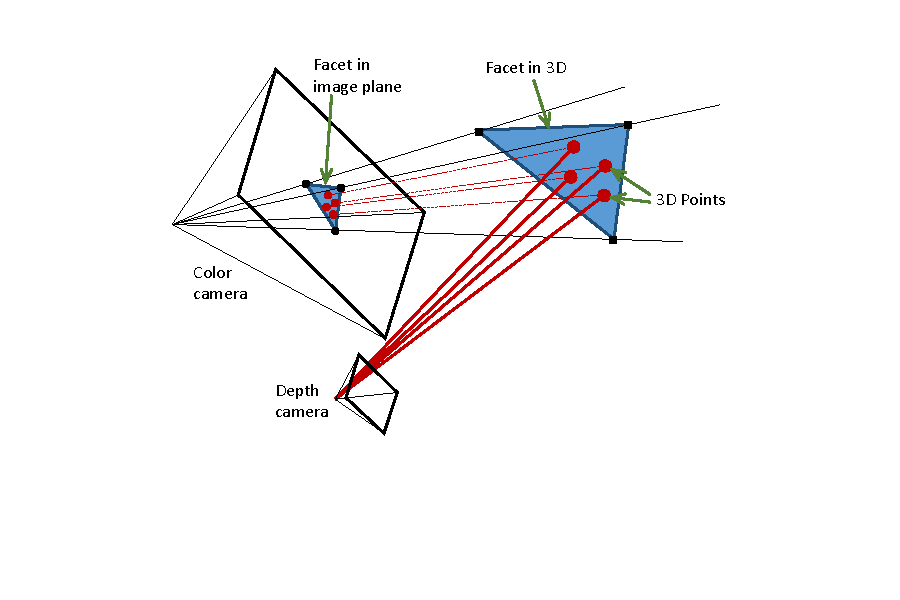
\includegraphics[trim=80 70 70 20,clip,width=0.95\linewidth]{Figures/pointFittingConcept}
\end{center}
   \caption{The parallel and adjacent color and depth cameras are shown as pyramids denoting their fields of view, and their size difference illustrates their relative resolutions.  Three vertices in a color image define the rays on which the vertices of the corresponding $3$D object facet must lie.  This facet is fit using the the $3$D points projected out from the depth camera.}
\label{fig:facet}
\end{figure}

To associate depth pixels with facets, pixels in the depth camera are projected along their rays out into $3$D, and then they are projected into the color image.  A depth pixel, $\point_i$, is associated with the facet, $\mathcal{F}_i$, into which it projects in the color image, as illustrated in Figure~\ref{fig:facet}. 

To estimate the facet parameters from depth measurements we will express the depth points, $\point_i$, after they have been projected out and transformed into color camera coordinates, as a linear function of the vertices of its facet:
\beq  %see PlantMacros.tex
\point_i = \sum_{j\in\mathcal{F}_i} \alpha_j \vertex_j. \label{eq:point}
\eeq
Here $\mathcal{F}$ is the set of three vertex indices belonging to the facet, and $\alpha_j$ is the coefficient of vertex $\vertex_j$ as illustrated in Figure~\ref{fig:triangle}, and $\sum_{j\in\mathcal{F}}\alpha_j=1$.  This linear sum is valid if we make a local orthographic approximation for the projection of a facet.  It will be a good approximation as long as the facet size is small compared to is depth from the camera, which is true for most applications.  Substituting in depth-scaled homogeneous vectors, and taking the third row, we obtain an equation for the point depth, $\lambda_i$, in the color image:
\beq
\lambda_i = \sum_{j\in\mathcal{F}_i} \alpha_j \lambda_j. \label{eq:pointdepth}
\eeq

\begin{figure}
\begin{center}
   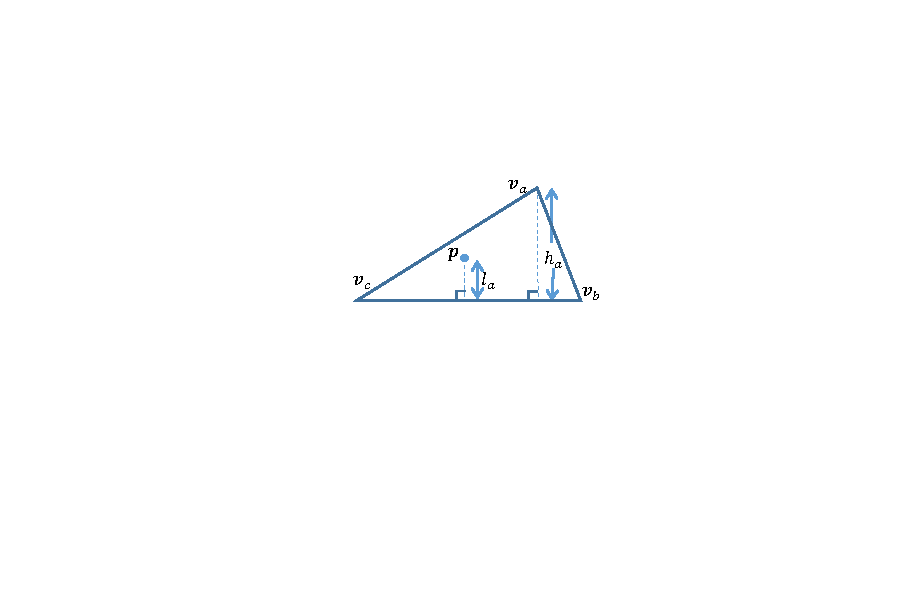
\includegraphics[trim=150 140 140 80,clip,width=0.5\linewidth]{Figures/TriangleParameterization}
\end{center}
   \caption{The coordinates of a point on a facet described by Eq.~(\ref{eq:point}) are the weighted linear sum of the three vertex coordinates.  The weight, $\alpha_a$, for vertex $\vertex_a$ is given by $\alpha_a = \frac{l_a}{h_a}$, the ratio of its perpendicular distance $l_a$ to the opposite edge to the vertex perpendicular distance $h_a$.  Analogous expressions describe $\alpha_b$ and $\alpha_c$. }
\label{fig:triangle}
\end{figure}

\subsection{Least Squares Depth}

Equation (\ref{eq:pointdepth}) gives the modeled depth of a point in terms of its facet vertices.  The depth camera will provide measured depths for each pixel, indicated as $\bar{\lambda}_i$, along with a standard deviation estimate $\sigma_i$ obtained from Eq.~(\ref{eq:sigma}).  Now this noise is along the depth ray, rather than the color camera ray, but since the depth and color cameras are close together compared to the distance to target, these rays are close to parallel and we assume $\sigma_i$ is a good measure along the camera ray.  With this approximation, the weighted least squares cost between measured and predicted depth is:
\beq
E_{depth}(\vlambda_{\vertex}) = \sum_{i\in\mathcal{D}} \|  \bar{\lambda}_i -  \sum_{j\in\mathcal{F}_i} \alpha_j \lambda_j \|^2_{\sigma_i^2}, \label{eq:meshleastsquares}
\eeq
where $\mathcal{D}$ is the set of depth pixels that project onto the target.  The L2 norm is weighted with the inverse variance of each point.  Minimizing this for $\vlambda_{\vertex}$, the set of all vertex depths, is a straightforward linear calculation.  


\subsection{Regularization}

Prior models on surface properties can be incorporated into the mesh via regularization and in so doing reduce the impact of noise.  In our application leaf surfaces are generally smoothly curved with few sharp edges.  We propose a regularization term that penalizes an approximate measure of curvature between pairs of facets: 
\beq
E_{reg}(\vlambda_v) = w\sum_{adj(i,j)} \| \frac{\cos(\normal_i\cdot\normal_j)^{-1}}{s_a+s_b} \|^2. \label{eq:reg}
\eeq
Here the sum is over all pairs of normals, $\normal_i$ and $\normal_j$, whose facets share an edge and hence are adjacent.  The numberator is the angle between the facet normals, $\theta$. The denominator is made from components shown in Fig.~\ref{fig:regularization}($a$) and it approximates the arc length, $s$ in the formula for curvature $k=\frac{\theta}{s}$.  $w$ is a weight controlling the level of smoothing.  By penalizing high curvatures the mesh can filter out strong noise.

It is also useful to have a linear regularization function.  Some vertices are insufficiently constrained the matrix inversion suffers from loss of full rank.  This tends to happen when facets are small enough that a number of them have no depth pixels projecting into them.  Adding a linear regularization term between pairs of facets will ensure that the coefficient matrix maintains full rank during least squares.

\begin{figure}
\begin{center}
\begin{tabular}{c}
   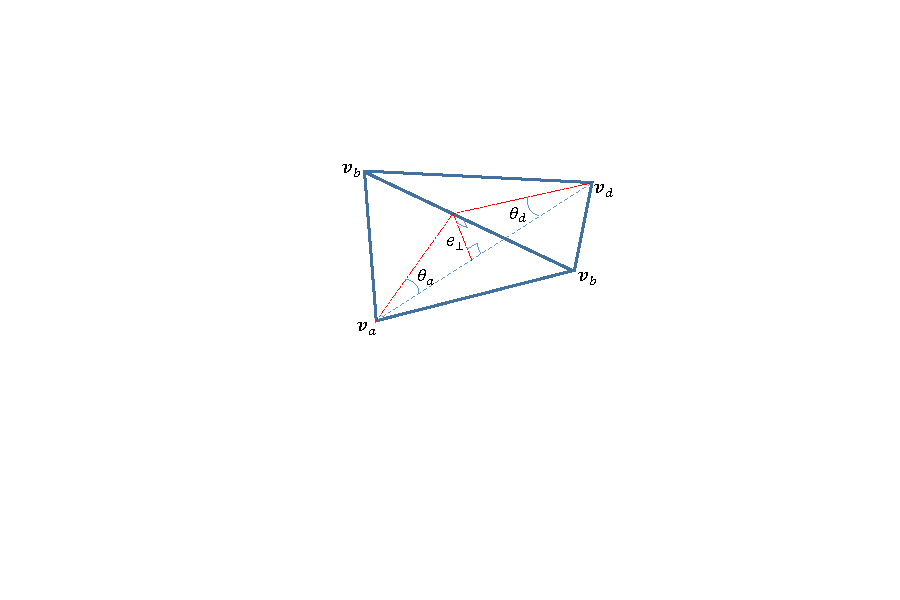
\includegraphics[trim=140 110 130 70,clip,width=0.6\linewidth]{Figures/adjacentFacets} \\
   ($a$) \\
   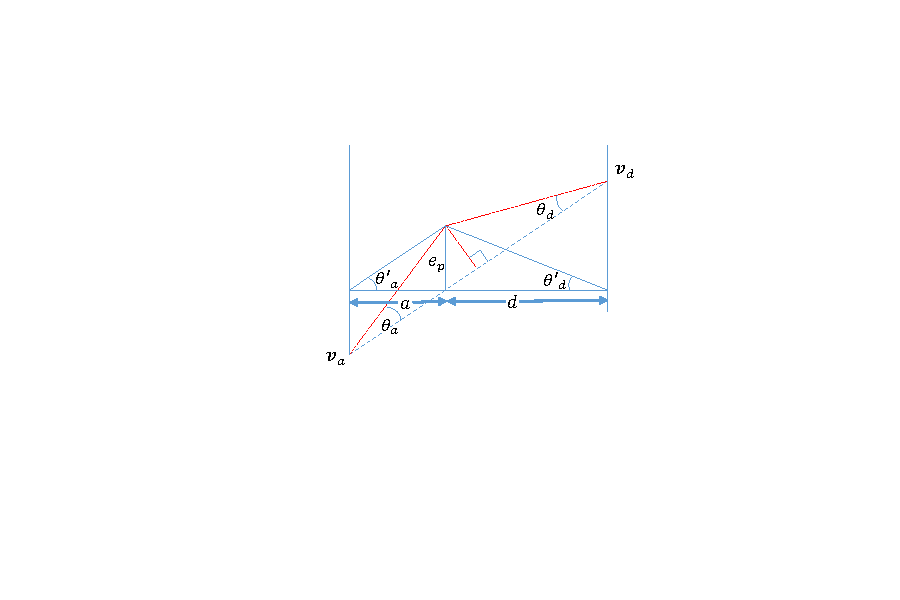
\includegraphics[trim=140 110 140 80,clip,width=0.65\linewidth]{Figures/adjacentApprox} \\
   ($b$) \\
\end{tabular}
\end{center}
   \caption{($a$) The angle between adjacent facet normals used in Eq.~(\ref{eq:reg}) can also be calculated as the sum of the angles subtended by $e_\perp$, namely: $\theta = \theta_a+\theta_d$. ($b$) An alternative is to use $\theta'_a$  and $\theta'_d$ as these can be calculated using the image projection of the facets, along with the depths of the vertices. }
\label{fig:regularization}
\end{figure}

We created an alternative linear regularization that uses an approximation to the angle between adjacent facets.  Figure~\ref{fig:regularization}($a$) illustrates that the angle between two adjacent facets is given by $\theta = \theta_a+\theta_d$, the angles subtended by $e_\perp$, the perpendicular distance between lines through opposite vertices of the (non-planar) quadrilateral formed by the two facets.  Instead we use the projection of the quadrilateral in the image, find the intersection of the lines between opposite vertices, and calculate the depth distance along this intersection ray $e_p = \frac{a\lambda_a+d\lambda_d}{a+d} - \frac{b\lambda_b+c\lambda_c}{b+c}$, where $a$, $b$, $c$ and $d$ are image distances along the edges joining the intersection point to the respective vertices.  Finally we use the tangent of the angles in the regularization to obtain:
\beq
\begin{array}{rcl}
E_{lin}(\vlambda_v) & = & w_l\sum_{adj(i,j)}  \|\tan(\theta'_{ai})\|^2 + \|\tan(\theta'_{di})\|^2 \\
           & = & w_l\sum_{adj(i,j)} \|\frac{e_p}{a_i}\|^2 + \|\frac{e_p}{d_i}\|^2. \label{eq:linreg} \\
\end{array}
\eeq
Again the sum is over all pairs of adjacent facets, and $w_l$ is the weighting term.  We found that these pairwise regularization terms performed better than Laplacian smoothing~\cite{Kobbelt:1998}.

\subsection{Algorithm}

The algorithm steps are:
\begin{enumerate}
\item Filter pixels occluded using Eq.~(\ref{eq:occluded})
\item Segment and build a planar mesh, see section~\ref{sec:colormesh}
\item Perform linear least squares for vertex depths, $\vlambda_v$, by minimizing $E_{depth}(\vlambda_{\vertex})+E_{lin}(\vlambda_v)$.
\item Refine $\vlambda_v$ by minimizing $E_{depth}(\vlambda_{\vertex})+E_{reg}(\vlambda_v)$.
\end{enumerate}

